
\documentclass[submit,techrep,noauthor,english]{ipsj}
\usepackage[dvipdfmx]{graphicx}
\usepackage{url}

%%%% 6-8 pages (max 10 pages)
%%%% less than 2MB

\def\Underline{\setbox0\hbox\bgroup\let\\\endUnderline}
\def\endUnderline{\vphantom{y}\egroup\smash{\underline{\box0}}\\}
\def\|{\verb|}
%
\long\def\comment#1{}
%

\begin{document}

\title{Is Japanese HPC another Galapagos?\\
- Interim Report of MPI International Survey -}

\affiliate{RCCS}{Riken-CCS}
\affiliate{UT}{University of Tennessee}
\affiliate{Inria}{Inria}

\author{Atsushi Hori}{RCCS}[ahori@riken.jp]
\author{George Bosilca}{UT}[bosilca@icl.utk.edu]
\author{Emmanuel Jeannot}{Inria}[emmanuel.jeannot@inria.fr]
\author{Takahiro Ogura}{RCCS}[t-ogura@riken.jp]
\author{Yutaka Ishikawa}{RCCS}[yutaka.ishikawa@riken.jp]

\begin{abstract}
We have been conducting questionnaire survey targeting MPI users of
whole world.  At the time of this writing, we get more than 800
answers from more than 40 countries.
We analyzed the currently available answers and have found some
interesting results which indicate that the Japanese MPI users are
different from the MPI users of the rest of the world. This paper focuses
on those possible specificities of Japanese MPI users and warns
the future of Japanese HPC community based. Since the survey is still
open and accepting answers, this is an interim report of the survey.
The word ``Galapagos'' in the title is widely used in Japan to
indicate something special which is though to be endangered%
\footnote{The analogy between Galapagos and Japan is that both consist
  of islands and species (technologies) evolves independently.}.  
\end{abstract}

\maketitle

\section{Overview}

In 2017, ECP\cite{ECP} conducted a survey for MPI users in the ECP
project to reveal how MPI would/should be integrated with ECP
applications in the future\cite{osti_1462877}.  It ws a coincidence
that another survey was conducted in Japan targeting HPCI\cite{HPCI}
users which included some MPI questions\cite{hpci-user-survey}.  If
both questionnaire surveys would have the same question(s), then we could
compare the answers to reveal the differences between US and
Japan. Unfortunately we could find only one similar question
related to MPI in both surveys.

We decided to conduct another MPI survey targeting MPI users of the
whole world. MPI is widely used vehicle for high-performance
computing, hoping we could find the differences of MPI users by
countries and/or regions of the world.

This project is being carried on by JLESC\cite{JLESC} which is an
international research collaboration framework. The international
nature of this survey matches the concept of JLESC. Each co-author is
a member of JLESC organizations and responsible for the country and/or
region where he belongs. 

\begin{table}[htb]%
\begin{center}%
\caption{Survey Comparison}\label{tab:comparison}%
\begin{tabular}{c|ccc}%
\hline%
Survey & Target & \# Questions & \# Answers \\%
\hline%
ECP  & US & 64 (max.) & 77 \\
HPCI & Japan & 75 (max.) & 105 \\
\hline
Our survey & International & 30 & 800+ \\
\hline%
\end{tabular}%
\end{center}%
\end{table}%

Our MPI International Survey, ECP survey, and HPCI survey are
summarized in Table~\ref{tab:comparison}. The major differences
between our survey and the others are;

\begin{description}
\item[Target]
  The ECP survey targeted ECP members who are leading researchers and
  application developers in USA. The HPCI survey targeted HPCI users
  who are programming HPC applications and using Japanese
  supercomputers. Thus, both surveys targeted high-end users. 
\item[Number of answers]
  The number of answers ECP survey and HPCI survey are 77 and 105,
  respectively. Because of the wider target of our survey, in terms of
  MPI expertise of participants on a global scale, the expected number of
  answers would be larger than those of preceding surveys.
\end{description}

As a result of our survey, although it is still accepting answers, we
got 800+ answers from 40+ countries at the time of this writing.  This
number of answers allows us to conduct cross-tab analysis between
questions on each countries and/or regions.

\section{Questionnaire}

\subsection{Design}

The points we kept in our mind while we were designing the
questions are; 

\subsubsection*{Number of questions}
This must be less than around 30 to keep  participants
concentrated\footnote{This project is one of the JLESC
  project\cite{JLESC} and 
  this number was advised by Prof. Marshall Scott Poole at Illinois Univ.,
  and Prof. Iftekhar Ahmed at Univ. of North Texas, they are also the
  members of JLESC\cite{JLESC}, from their social science viewpoints.}.
The maximum numbers of questions in the ECP survey and HPCI survey are
64 and 75, respectively. Thus, the number of questions in this survey
is far less than those.  We focused on MPI itself to reduce the number
of questions.  For example, the questions asking about the tools are
intentionally excluded simple because this may add several tens of
questions. Another survey must be conducted for the topics not
included in our survey.

\begin{description}
\item[Easy-to-answer]
We designed our questions to minimize the stress of participants as
much as possible. None of our questions requires free descriptive
answers. Additional investigations and/or efforts are minimized. If we
would ask participants about the LOC (lines of code) they have ever
programmed, they would run the {\tt wc} command on their programs.  

\item[Minimizing ambiguity]
The above LOC question may introduce ambiguity into its answer; 1)
large numerical applications may have more than hundreds thousand LOC,
but the LOC for MPI function calls is much less than the whole LOC, 2)
participants might or might not include the LOC of supplementary code
such as {\tt Makefile}, {\tt configure} and others. 
We also tried not to have MPI-IO related questions because of not only
the number of questions but also the difficulty for novice MPI users
to identify the root cause; the MPI standard, MPI implementation,
MPI-IO implementation, system configuration, or underlying file
system. 
\end{description}

\begin{table}
  \caption{Questions}\label{tab:questions}
\begin{description}
\tiny\bf
\item{Q1:} What is your main occupation?
\item{Country:} Select main country or region of your workplace in
  past 5 years 
\item{Q2:} Rate your overall programming skill (non-MPI programs) 
\item{Q3:} Rate your MPI programming skill
\item{Q4*:} What programming language(s) do you use most often?
\item{Q5:} How long have you been writing computer programs
  (incl. non-MPI programs)? 
\item{Q6:} How long have you been writing MPI programs?
\item{Q7*:} Which fields are you mostly working in?
\item{Q8*:} What is your major role at your place of work?
\item{Q9:} Have you ever read the MPI standard specification document?
\item{Q10*:} How did you learn MPI?
\item{Q11*:} Which MPI book(s) have you read?
\item{Q12*:} Which MPI implementations do you use?
\item{Q13:} Why did you choose the MPI implementation(s)?
\item{Q14*:} How do you check MPI specifications when you are writing
  MPI programs? 
\item{Q15:} What is the most difficult part of writing an MPI program?
\item{Q16*:} Which MPI features have you never heard of?
\item{Q17*:} What aspects of the MPI standard do you use in your
  program in its current form? 
\item{Q18*:} Which MPI thread support are you using?
\item{Q19*:} What are your obstacles to mastering MPI?
\item{Q20:} When you call an MPI routine, how often do you check the
  error code of the MPI routine  (excepting MPI-IO)? 
\item{Q21:} In most of your programs, do you pack MPI function calls
  into their own file or files to have your own abstraction layer for
  communication? 
\item{Q22*:} Have you ever written MPI+''X'' programs?
\item{Q23:} Is there any room for performance tuning in your MPI
  programs? 
\item{Q24*:} What, if any, alternatives are you investigating to
  indirectly call MPI or another communication layer by using another
  parallel language/library? 
\item{Q25:} If there were one communication aspect which is not enough
  in the current MPI could improve the performance of your
  application, what would you prioritize? Or is MPI providing all the
  communication semantics required by your application? If not, what
  is missing? 
\item{Q26*:} Is MPI providing all the communication semantics required
  by your application? If not, what is missing? 
\item{Q27*:} What MPI feature(s) are NOT useful for you application? 
\item{Q28:} Do you think the MPI standard should maintain backward
  compatibility? 
\item{Q29:} In the tradeoff between code portability and performance,
  which is more or less important for you to write MPI programs? 
\end{description}
\end{table}

\subsection{Questions}

Table~\ref{tab:questions} shows all questions in our survey. The
number of questions is 30 including a question asking the country of
participants. Note that this question does not ask the nationalities
of participants but workplace for recent 5 years. The answers of this
question are used to categorize answers into the countries and/or
regions in the following analysis sections. The question suffixed by
an asterisk (*) allow participants to select multiple answers. 

\section{Distribution}

We conducted prerelease testing on MPI Forum\cite{mpi-forum} attendees
and Riken-CCS researchers. An interview with a R-CCS
researcher was also conducted to debug and tune the questions at the
very final stage of the questionnaire design.

The questionnaire is implemented by using Google Forms and distributed
by sending e-mails to major mailing lists including {\tt
  hpc-announce}. We started distributing the survey from 17th of
February, 2019. All data in this paper is as of 10th of
May. Figure~\ref{fig:timeseries} shows the number of answers since then.

Soon after we started distribution, we realized that the major
mailing-lists (e.g., {\tt hpc-announce}) did not work well as we
expected. So we started asking our friends to help us to distribute
the survey to their local communities. In Figure~\ref{fig:timeseries},
the number of answers increases stepwise. This is because our friends
re-distributed the survey to their local communities at each step. 

\begin{figure}[htb]
\begin{center}
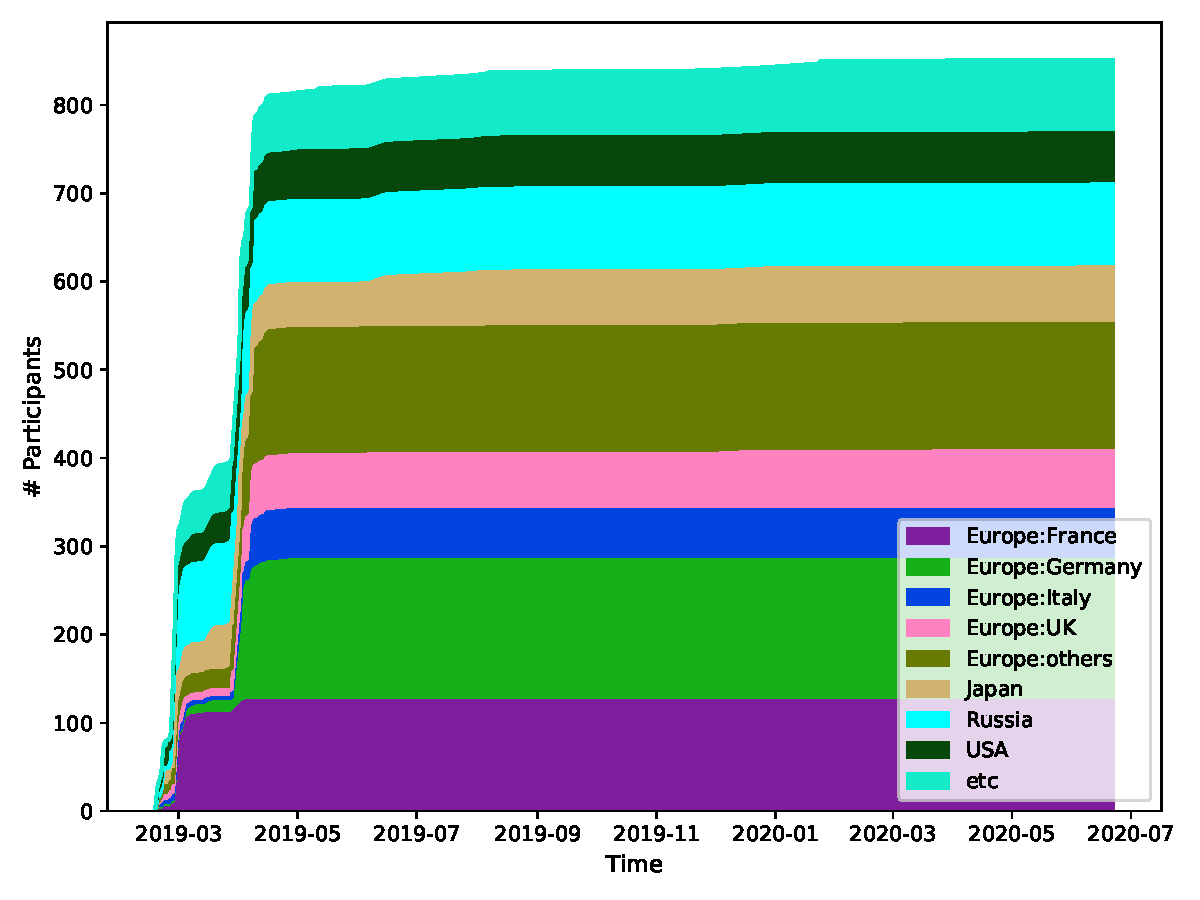
\includegraphics[width=9cm]{../pdfs/TimeSeries.pdf}
\caption{Time series}
\label{fig:timeseries}
\end{center}
\end{figure}

The answers are automatically collected by Google Forms. So a
questionnaire survey in this way (using Google Forms and sending
e-mails) is very easy, fast, and no charge.  However, we could have 
answers only from the mailing-lists and these responses may have the
possibility of having some differences from the ones obtained by a
random sampling way. Thus, our survey may include some bias and be
different from ideal responses representing statistical population.  

We developed a Python program to analyze the resulting CSV files. For
cross-tab analysis, this program outputs graphs of all possible
combination of two questions excepting the ones where both questions
allow to have multiple answers. All graphs in this paper were created
by this Python program. 

\section{Profile of Participants}\label{sec:profile}

Table~\ref{tab:countries} shows the number of answers of top-10
countries. It should be noted that the question asked the workplaces
of participants for recent 5 years, not the nationality. As of this
writing, we got only 4 answers from China. This is because Chinese
government does not allow its people to access Google. 

\begin{table}[htb]%
\begin{center}%
\caption{Top 10 Countries}\label{tab:countries}%
\begin{tabular}{c|l|r}%
\hline%
Rank & Country & \# Answers \hspace{5mm} \\%
\hline%
1 & Germany 	& 159 \hspace{8mm} \\%
2 & France 	& 125 \hspace{8mm} \\%
3 & Russia 	& 94 \hspace{8mm} \\%
4 & UK 		& 62 \hspace{8mm} \\%
5 & USA 	& 57 \hspace{8mm} \\%
6 & Italy 	& 57 \hspace{8mm} \\%
7 & Japan 	& 51 \hspace{8mm} \\%
\hline
8 & Switzerland & 40 \hspace{8mm} \\%
9 & Korea, South & 27 \hspace{8mm} \\%
10 & Austria 	& 26 \hspace{8mm} \\%
\hline%
\multicolumn{3}{c}{41 countries, 817 answers} \\%
\end{tabular}%
\end{center}%
\end{table}%

Table~\ref{tab:top500} shows the top-10 countries of the system share
in Top500 list as of November 2018\cite{Top500}. Comparing
Table~\ref{tab:countries} and \ref{tab:top500}, it is ver obvious that
the numbers of answers from China, USA, Japan and Canada in our survey
do not reflect the system share in Top500.  This is the reason not to
close the survey until the gap between Table~\ref{tab:countries} and
\ref{tab:top500} becomes close enough.

\begin{table}[htb]%
\begin{center}%
  \caption{Top 10 Countries in Top500 System Share\cite{Top500}}
  \label{tab:top500}%
\begin{tabular}{c|l|c}%
\hline%
Rank & Country & System Share [\%] \\%
\hline%
1 & China & 45.4 \\%
2 & USA & 21.8 \\%
3 & Japan & 6.2 \\%
4 & UK & 4.0 \\%
5 & France & 3.6 \\%
6 & Germany & 3.4 \\%
7 & Ireland & 2.4 \\%
8 & Canada & 1.8 \\%
9 & Italy & 1.2 \\%
10 & Korea, South & 1.2 \\%
\hline%
\multicolumn{3}{r}{\tiny As of November 2018} \\
\end{tabular}%
\end{center}%
\end{table}%

From this time onward, the countries and regions (a set of countries)
having more than 50 answers are focused in this paper (the top-7
countries in Table~\ref{tab:countries}).  The countries
having less number of answers may contain large bias and they are
inadequate for cross-tab analysis. 

Figure~\ref{fig:occupation} shows the survey result of Q1 in
Table~\ref{tab:questions} asking the participants'
occupations. Although we can see some diversities, most answers,
around 80\%, come from research organizations (universities and
governmental research institute).  We do not think this
diversities did not reflect the characteristics of the countries, but
they comes from the biased questionnaire distribution. 

\begin{figure}[htb]
\begin{center}
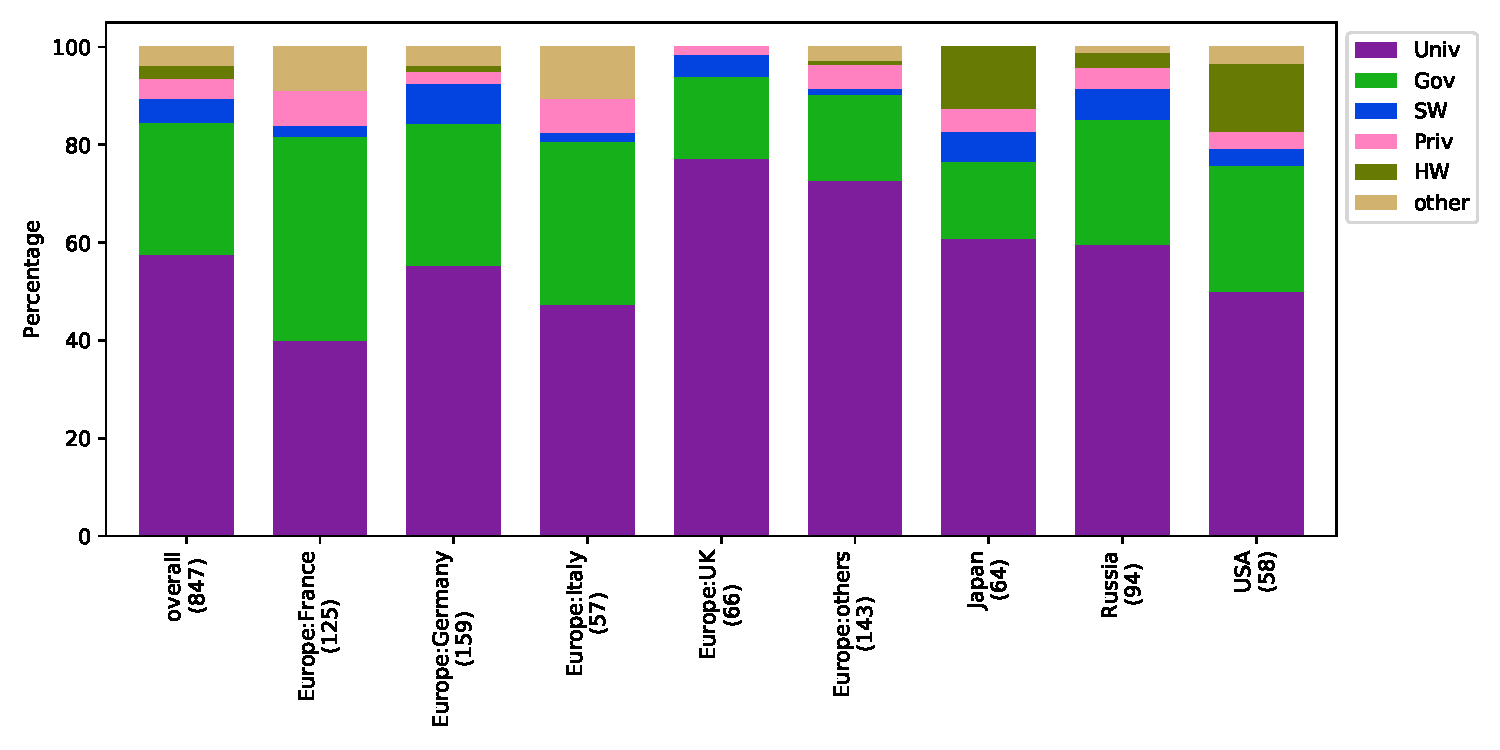
\includegraphics[width=9cm]{../pdfs/Q1.pdf}
  \vspace{-8mm}
  \caption{Q1: Occupation\\
    {\bf Univ}: University, {\bf Gov}: Governmental institue,
    {\bf Priv}: Private institute, {\bf SW}: SW vendor,
    {\bf HW}: HW vendor}
  \label{fig:occupation}
\end{center}
\end{figure}

These answerers' profile may bias the analysis inf the 
following sections. Thus, readers must keep in mind on the above
situations.
The following sections will show the results of analysis of our survey
data. In this paper, we chose the ones which reveals the specificities
of Japan. 

\section{Simple Tabulation}\label{sec:simple-tab}

Figure~\ref{fig:q5} shows the simple-tab results asking how many years
for writing programs (including MPI) and Figure~\ref{fig:q6} shows the
results asking how many years for writing MPI programs. Each bar
represents a country or region having more than 50 answers. ``whole''
represents the whole data and ``Europe:other'' represents the sum of
other European countries. The numbers
following the column titles represent the number of answers of that
country/region and the number of total answers of the question.

\begin{figure}[htb]
\begin{center}
  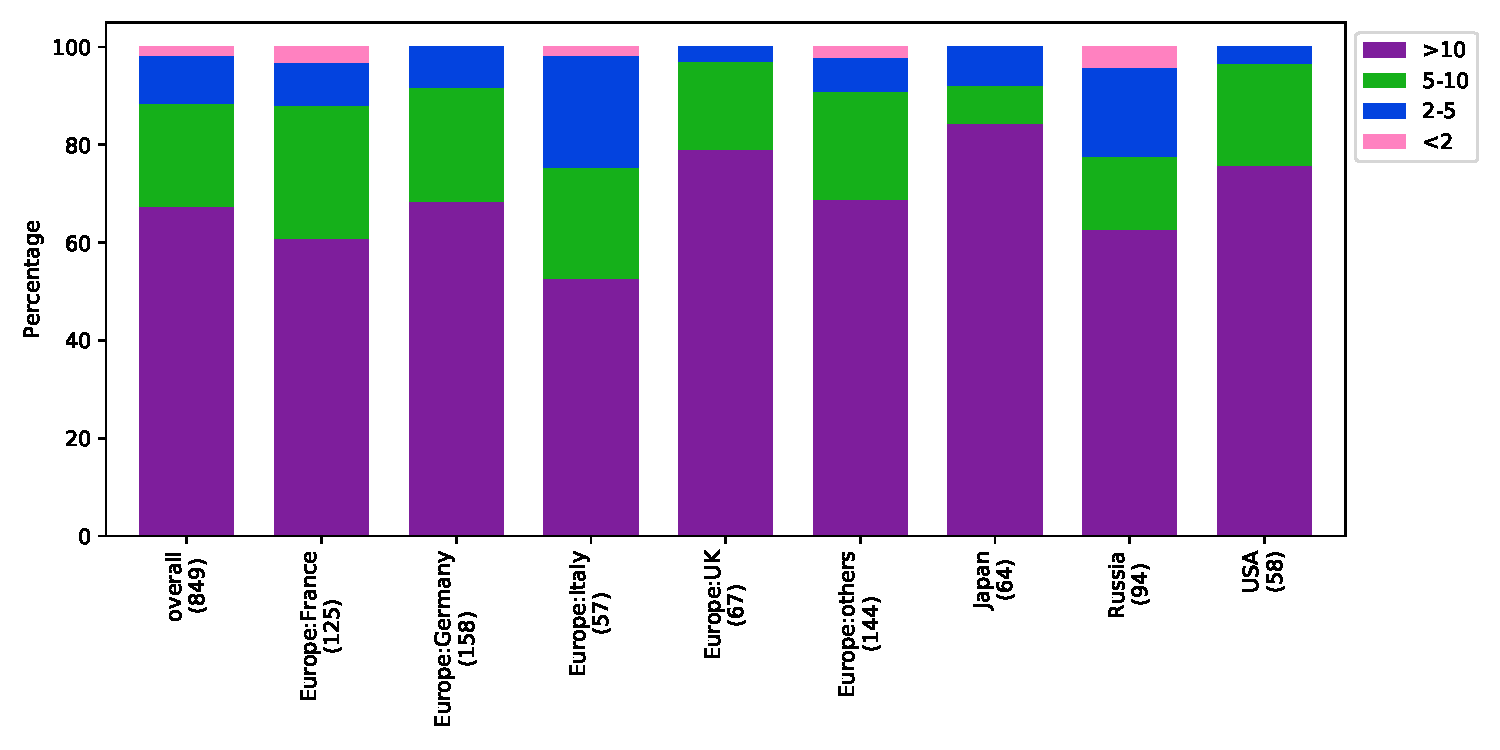
\includegraphics[width=9cm]{../pdfs/Q5.pdf}
  \vspace{-8mm}
\caption{Q5: Programming Experience}
\label{fig:q5}
\end{center}
\end{figure}

\begin{figure}[htb]
\begin{center}
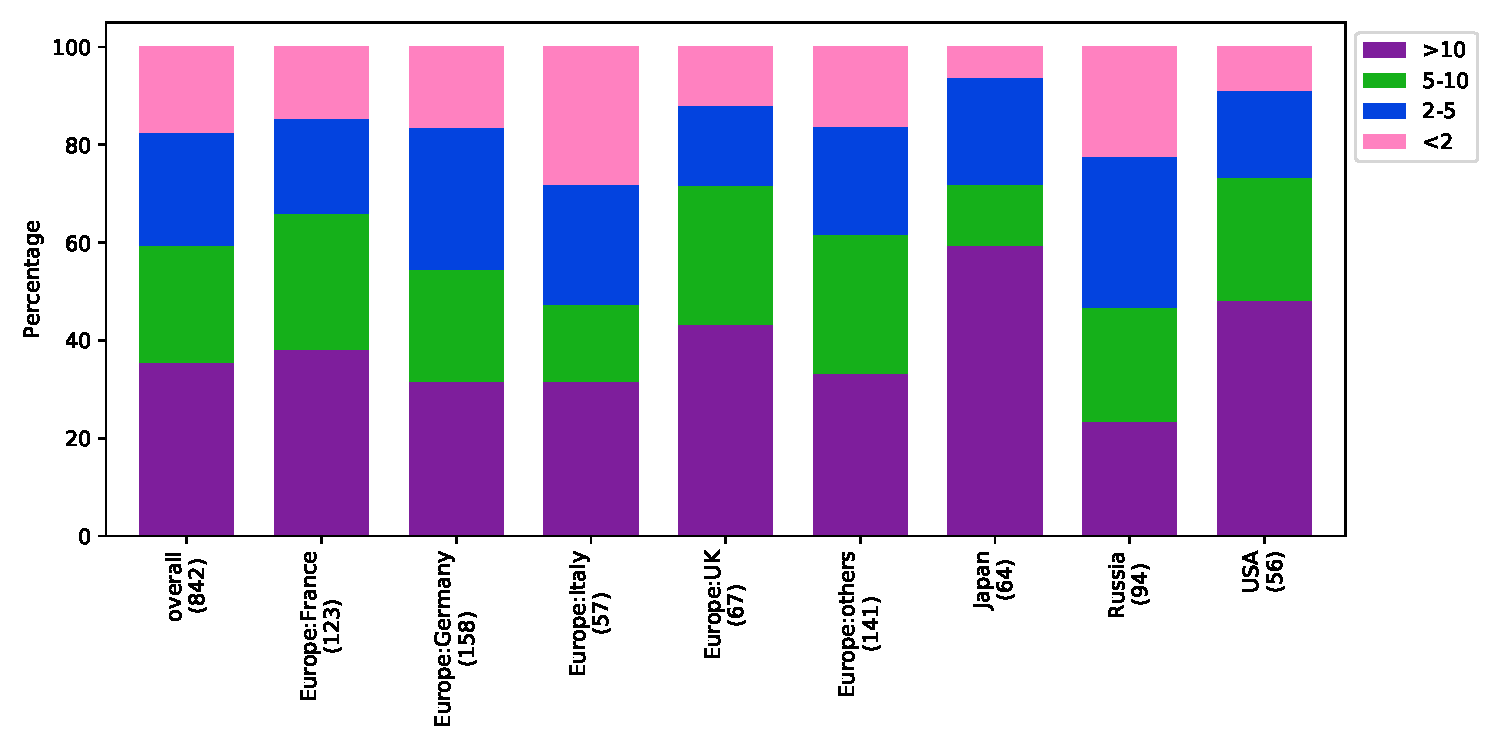
\includegraphics[width=9cm]{../pdfs/Q6.pdf}
  \vspace{-8mm}
\caption{Q6: MPI Experience}
\label{fig:q6}
\end{center}
\end{figure}

It is very interesting that the Japan's percentages of writing MPI and
non-MPI programs more than 10 years are highest among the
others. This looks like the Japanese HPC researchers and programmers
are well-experienced. However, it can also be said that only little
researchers and programmers are writing MPI programs. Contrastingly
in Germany and Russia cases, novice users, intermediate users, and
experienced users are almost equally distributed.  These look like
ideal cases. 

\begin{figure}[htb]
\begin{center}
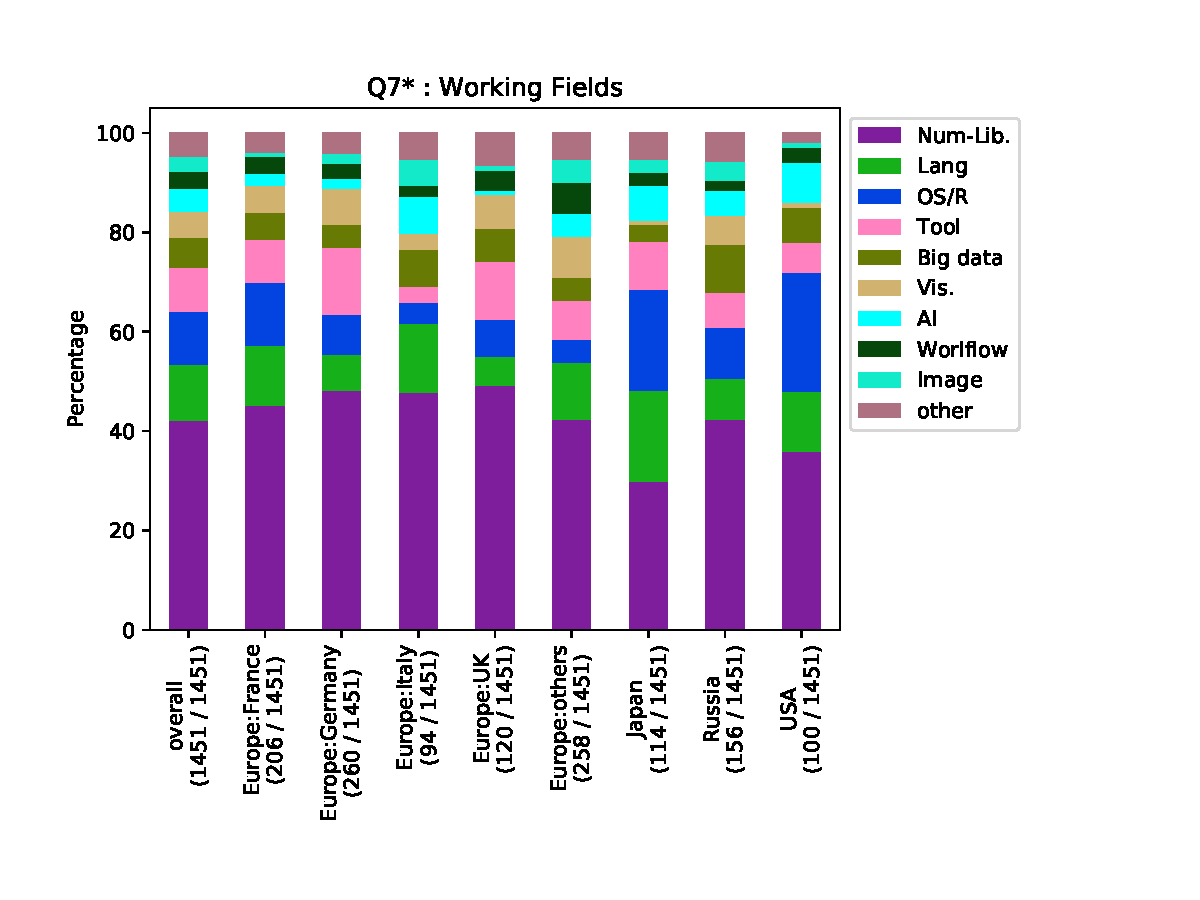
\includegraphics[width=9cm]{../pdfs/Q7.pdf}
  \vspace{-8mm}
\caption{Q7: Field}
\label{fig:q7}
\end{center}
\end{figure}

Figure~\ref{fig:q15} shows the answers asking about the MPI
difficulty. In Japan, the ratios of people having the difficulty for
debugging and tuning are the highest among the other countries. And
the ratios for algorithm selection and domain decomposition, which
are apparently higher levels than the levels of debugging and tuning,
are least among the other countries/regions.

\begin{figure}[htb]
\begin{center}
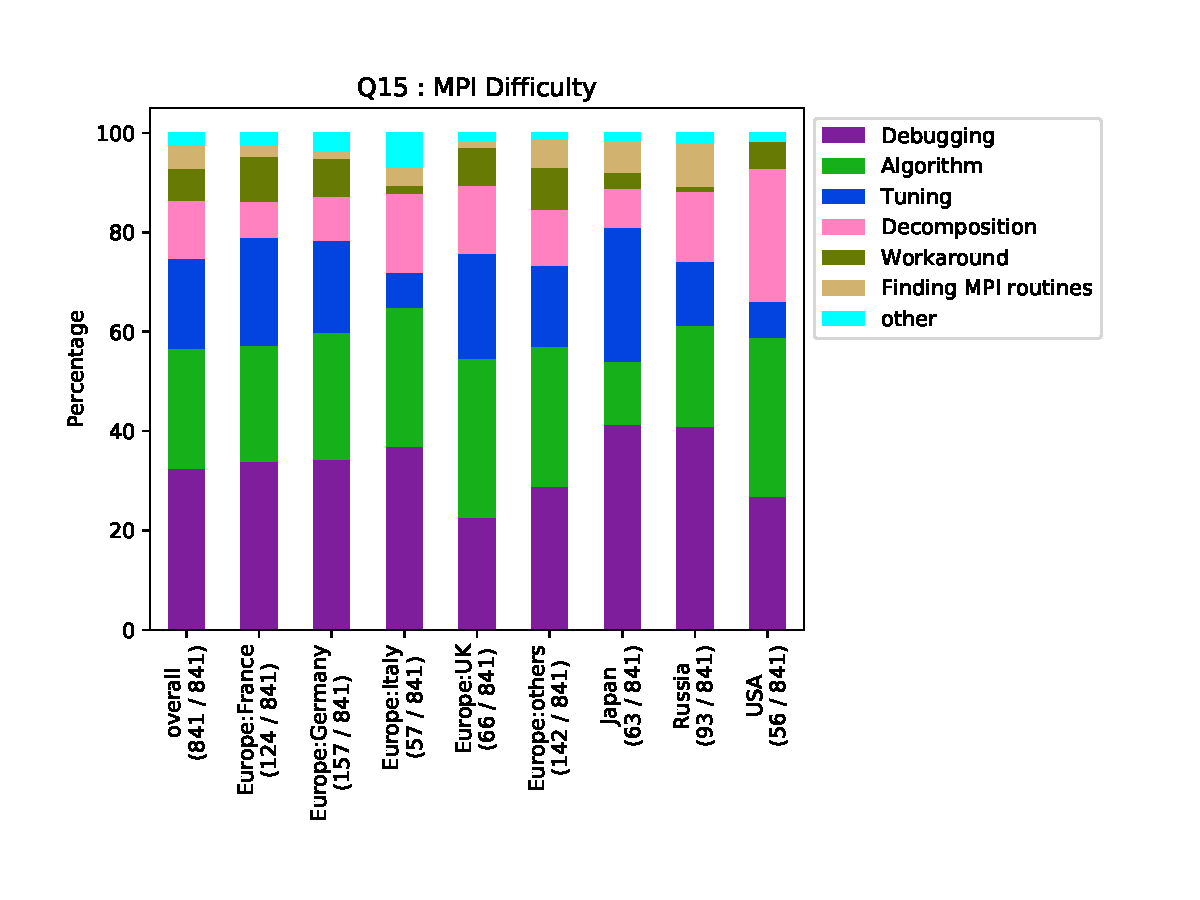
\includegraphics[width=9cm]{../pdfs/Q15.pdf}
  \vspace{-8mm}
\caption{Q15: Difficulty}
\label{fig:q15}
\end{center}
\end{figure}

These results may come from the role of
participants. Figure~\ref{fig:q8} shows the role of 
participants. Unlike the other countries, more Japanese MPI users are
working on research and development of OS and runtime, and less users
are working on tools. This Japan's specificity may affect the result
of Figure~\ref{fig:q5} and \ref{fig:q7}, because the OS and runtime
code are harder to debug and tune than that of applications in many
cases. It is also assumed that algorithm selection and domain
decomposition are the roles of its users. 

\begin{figure}[htb]
\begin{center}
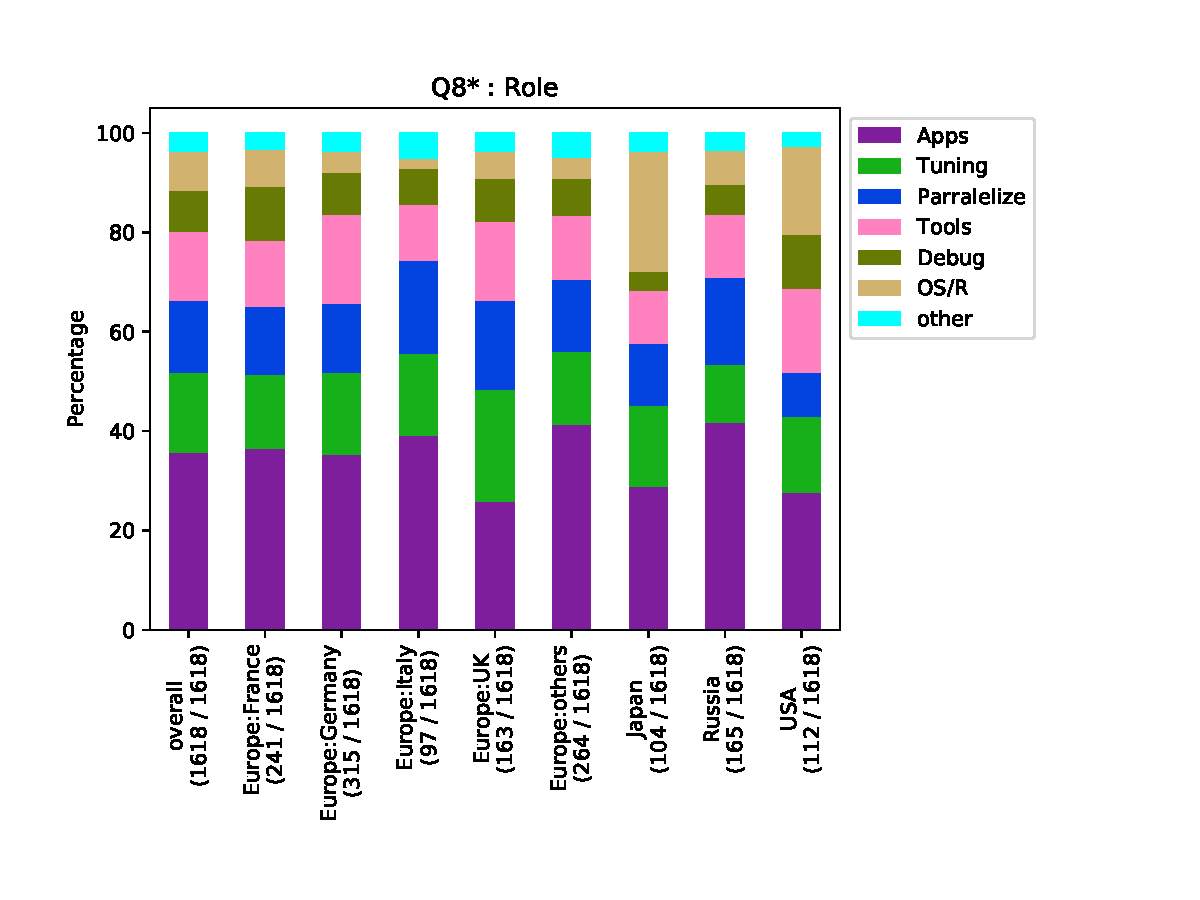
\includegraphics[width=9cm]{../pdfs/Q8.pdf}
  \vspace{-8mm}
\caption{Q8: Role}
\label{fig:q8}
\end{center}
\end{figure}

Figure~\ref{fig:q23} shows the result of asking the room for tuning in
participants' applications. As shown in this figure, Japan has the
lowest ratio of the answer ``My programs are (already) well-tuned.''
At the same time, Japan has the highest ratio of the answer
``Rewriting programs is too hard'' whereas they recognize the room for
tuning in their applications. Yes, we agree that rewriting a program
for tuning sometimes requires lots of work; for example, major data
structure changes may affect whole program.

\begin{figure}[htb]
\begin{center}
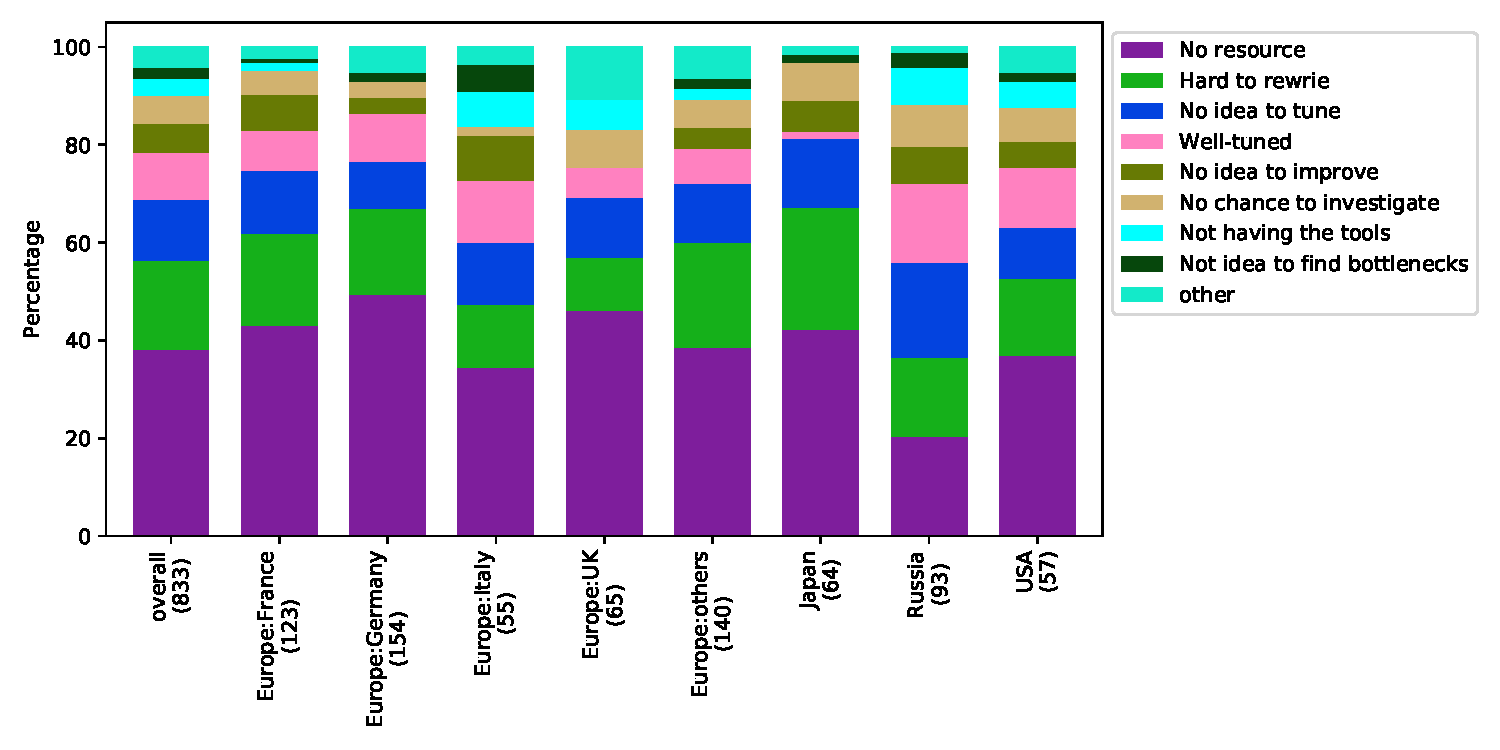
\includegraphics[width=9cm]{../pdfs/Q23.pdf}
  \vspace{-8mm}
\caption{Q23: Room for Tuning}
\label{fig:q23}
\end{center}
\end{figure}

In this question, there is another choice of ``I do not have
enough resource for tuning.'' What is the difference between the
answers of ``rewriting is too hard'' and ``not having enough
resource?'' Considering with the lowest ratio of ``My programs are
well-tuned'' answer, ``rewriting...'' answer sounds like a trouble or
{\it giving up thinking} while the latter one sounds more aggressive.

\section{Cross Tabulation}

The cross-tab graphs in this section are heatmap graphs. The
higher (darker) the value (color) of each cell, the higher the
frequency of the cell. There are nine graphs in this figure, each
graph represents a country or region. The lower-right graph is the
legend of these graphs serving as a color bar, too. The numbers in the
cells in the legend graph are percentages. The row(s) and column(s)
consisting only of the cells less than 4\% in all countries/regions
are omitted for readability.

\begin{figure}[htb]
\begin{center}
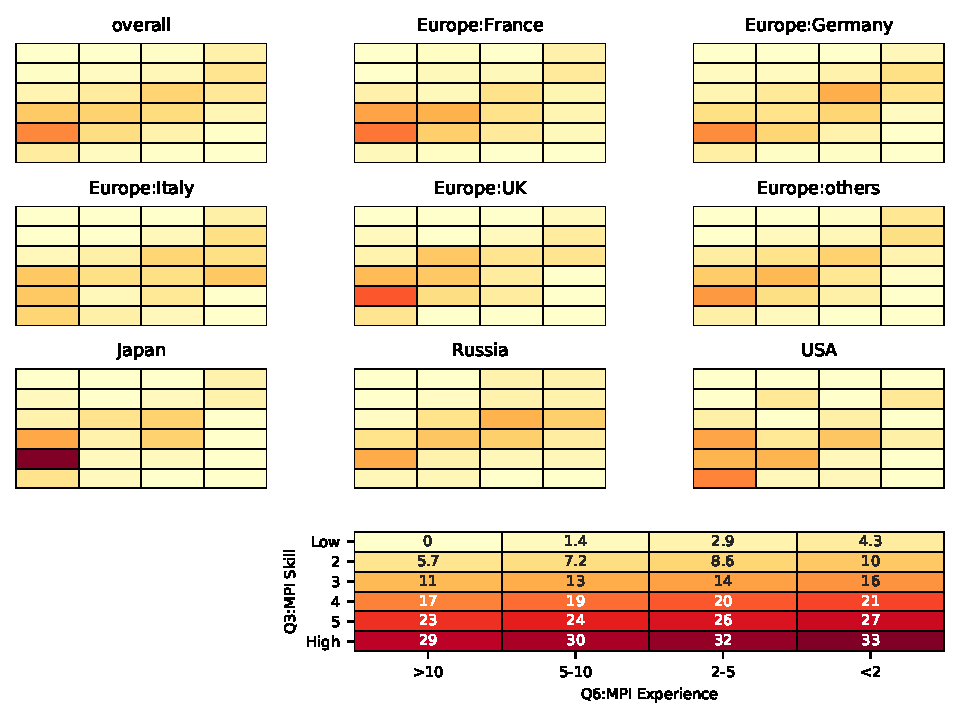
\includegraphics[width=9cm]{../pdfs/Q3-Q6.pdf}
\caption{Q3-Q6: MPI Skill and MPI Experience}
\label{fig:q3-q6}
\end{center}
\end{figure}

Figure~\ref{fig:q3-q6} shows cross-tab heatmap graphs between
Q3 (asking MPI skill) and Q18 (asking MPI experience). As shown in
this figure, Japanese answers are concentrated in the cell with the high
MPI skill of 5 (out of 6, larger the number, higher the skill) and
having more than 10 years of MPI experiences. In contrast to Japan,
although the Japan's high peak makes the peaks of the others lower and
hard to see, the peaks of the other countries are rather distributed. 

\begin{figure}[htb]
\begin{center}
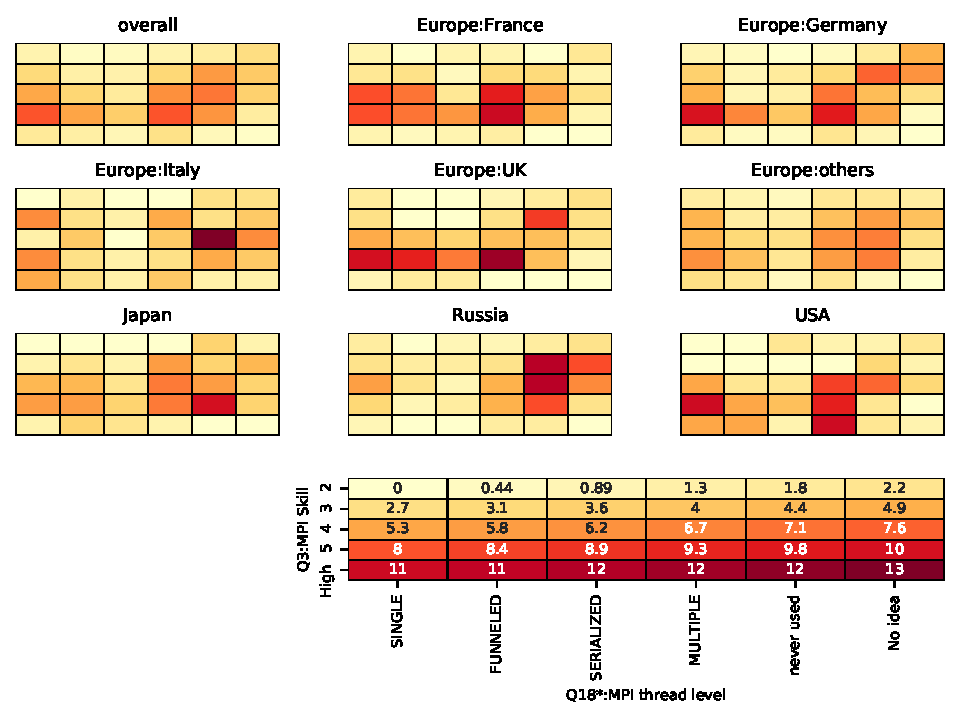
\includegraphics[width=9cm]{../pdfs/Q3-Q18.pdf}
\caption{Q3-Q18: MPI Experience and MPI Thread Level}
\label{fig:q3-q18}
\end{center}
\end{figure}

Figure~\ref{fig:q3-q18} shows the cross-tab graphs between
Q3 (asking MPI skill, again) and Q18 (asking MPI thread
level). There is a peak at 'Never used,' this means that many Japanese
participants do not explicitly call the {\tt MPI\_Init\_thread}
function.  The doubt here is why Japanese MPI {\em experts} do not
call the {\tt MPI\_Init\_thread} function. 
In contrast, in the Russian case, the ratio of ``Never used'' answer
increases when the  MPI skill decreases. In the USA case, the ratio of
using {\tt MPI\_THREAD\_MULTIPLE} increases when the MPI skill goes
up. Thus, the Japanese specificity comes to the front.

\section{Concerns about Japanese HPC}

In this section, we dare say our concerns about Japanese HPC. The
following two points are our hypothesises based on the results of our 
survey. Our survey might be biased and the hypothesises might be
wrong. But these are our warning messages if our hypothesises are
true. 

\subsection{Aged MPI users}

As shown in Figure~\ref{fig:Q5} and \ref{fig:Q6}, the most MPI users
in Japan have more experiences than the other countries. This might
sound good, but it is not good when you think about its future.  This
means there are only little {\em novice} MPI users in Japan.
Experienced Japanese MPI users decreases in the future.  We
call MPI users in Japan {\em aged}, not experienced. The reason of
this will be described in following subsection.

\subsection{Less effort on MPI programming}

In the previous section we discussed about another Japanese
specificity about the use of {\tt MPI\_Init\_thread} in
Figure~\ref{fig:q3-q18}. Considering with the aged MPI users in Japan,
one possible explanation of this is that they are still calling MPI
functions only appeared in the old MPI standard. And this hypothesis
can lead to the next hypothesis; they do not writing MPI programs from
the scratch, but changing existing MPI programs.

This new hypothesis is consistent with the result of Q15 asking MPI
programming difficulty. As discussed in Section~\ref{sec:simple-tab},
many Japanese participants have the difficulty with the low-level
program development; debugging and tuning, whereas they do not
dominate that much in the other countries or regions. If an MPI user 
tries to write a new MPI program, firstly they have to think about
parallel algorithm and domain decomposition. Bu many MPI users in
Japan do not suffer from these issues.

\subsection{Negative attitude to MPI programming}

On the question Q23 asking room for performance tuning, there is one
Japanese {\it other} answer; ``Yes, but it’s an MPI implementation
issue.'' This sounds like that the tuning effort is not his/her job
but MPI implementors. This answer is too negative and he/she does not
capture the nature of parallel programming at all.

\subsection{Are Japanese MPI users really expert?}

Taking int account of all above discussions, we dare say ``MPI users
in Japan may NOT be experts although they say so.'' They declare they
have long experiences with MPI in the Q6 question, but the other
questions in our survey reveal that they may not be. As the aged MPI
users fade away in the future, it is hard to deny that the Japanese
HPC will be in a big trouble. 

\section{Summary and Future Work}

We report an interim report of MPI International Survey. We designed
the questionnaire very carefully; 1) 30 questions, 2) easy-to-answer,
and 3) minimizing ambiguity. As of this writing we got more than 800
answers from more than 40 countries. In this paper, we focused on the
Japanese HPC situation though the questionnaire. Although the answers
might be biased, we warned the possibilities of critical situations
in Japanese HPC. These are two points; a) aged MPI researchers and
developers, b) less effort on MPI programming, and c) negative
attitude to MPI programming. 

Recently we opened a new survey site for those who cannot access
Google Forms by using Microsoft Forms, having the same questions and
answer choices. We will get answers from China who owns the most
powerful supercomputers. We are also trying to narrow the gap
described in Section~\ref{sec:profile}. 

We believe that this international survey in the JLESC framework worked
very well.  The other HPC related surveys which we excluded due to the
number of questions are planned to follow.

All survey data obtained by Google Forms and Microsoft Forms and the
Python program to draw graphs are open and can be downloaded from
GITHUB freely (\url{https://github.com/bosilca/MPIsurvey/}).

The URLs for the questionnaire are shown in
Figure~\ref{fig:QR-codes}. Again, the survey is open and accepting
answers. If you are interested in participating the survey, please
access one of the ULRs in this figure.

\begin{figure}[htb]
\begin{center}
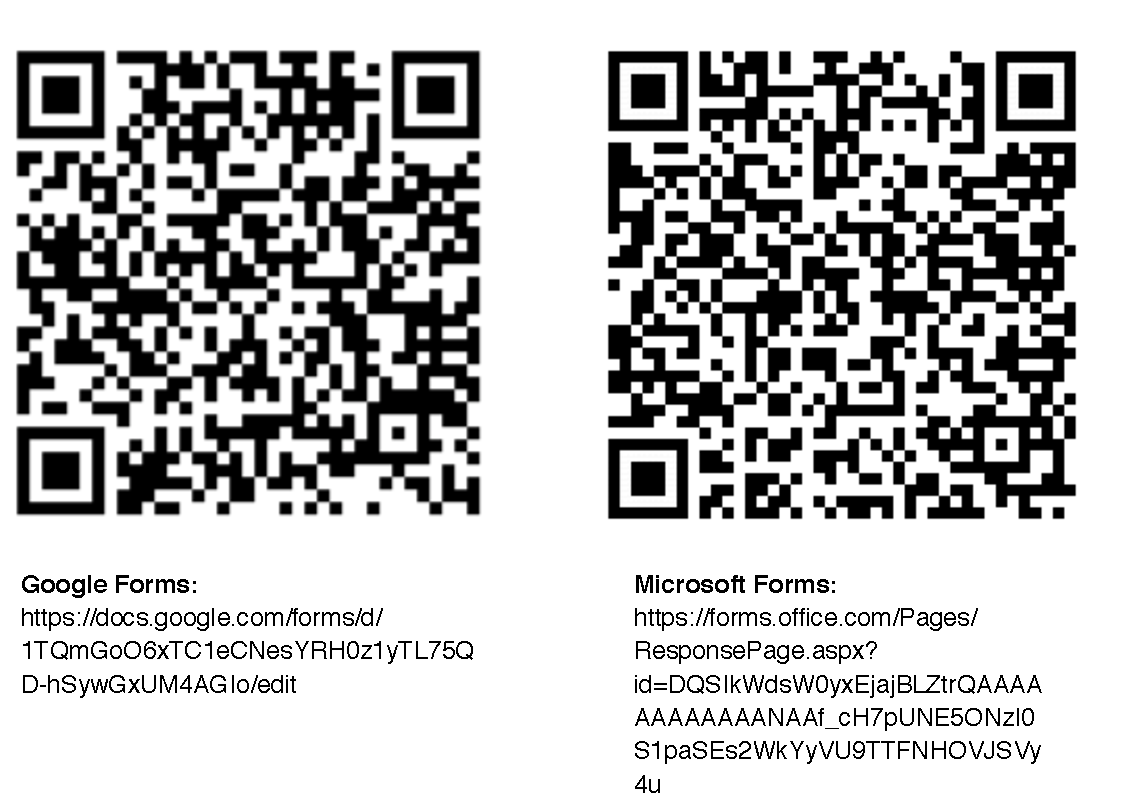
\includegraphics[width=8cm]{figs/QR-codes.pdf}
\caption{QR codes to access the survey}
\label{fig:QR-codes}
\end{center}
\end{figure}

\begin{acknowledgment}
  We thank to those who participated in this survey and those who
  helped us to distribute the survey to their local communities.\\
  This research is partially supported by the
  NCSA-Inria-ANL-BSC-JSC-Riken-UTK Joint-Laboratory for Extreme Scale
  Computing (JLESC, \url{https://jlesc.github.io/}).
\end{acknowledgment}


\bibliographystyle{ipsjsort-e}
\bibliography{../ref}

\end{document}
